\section{Istruzione utilizzo utente amministratore}

La seguente sezione fornirà indicazioni utili per il corretto utilizzo del software nel caso l'utente interessato sia l'amministratore.

\subsection{Login}
Il primo passo da effettuare è l'inserimento del proprio codice identificativo e password all'interno dei campi visualizzati nella pagina di login. Dopo aver premuto il pulsante di conferma, si sarà indirizzati alla pagina dedicata alle funzionalità di amministratore. Nel caso le credenziali inserite non risultino corrette, sarà visualizzato un messaggio d'errore e sarà quindi necessario inserire di nuovo i dati.
\begin{figure}[H]
    \centering
    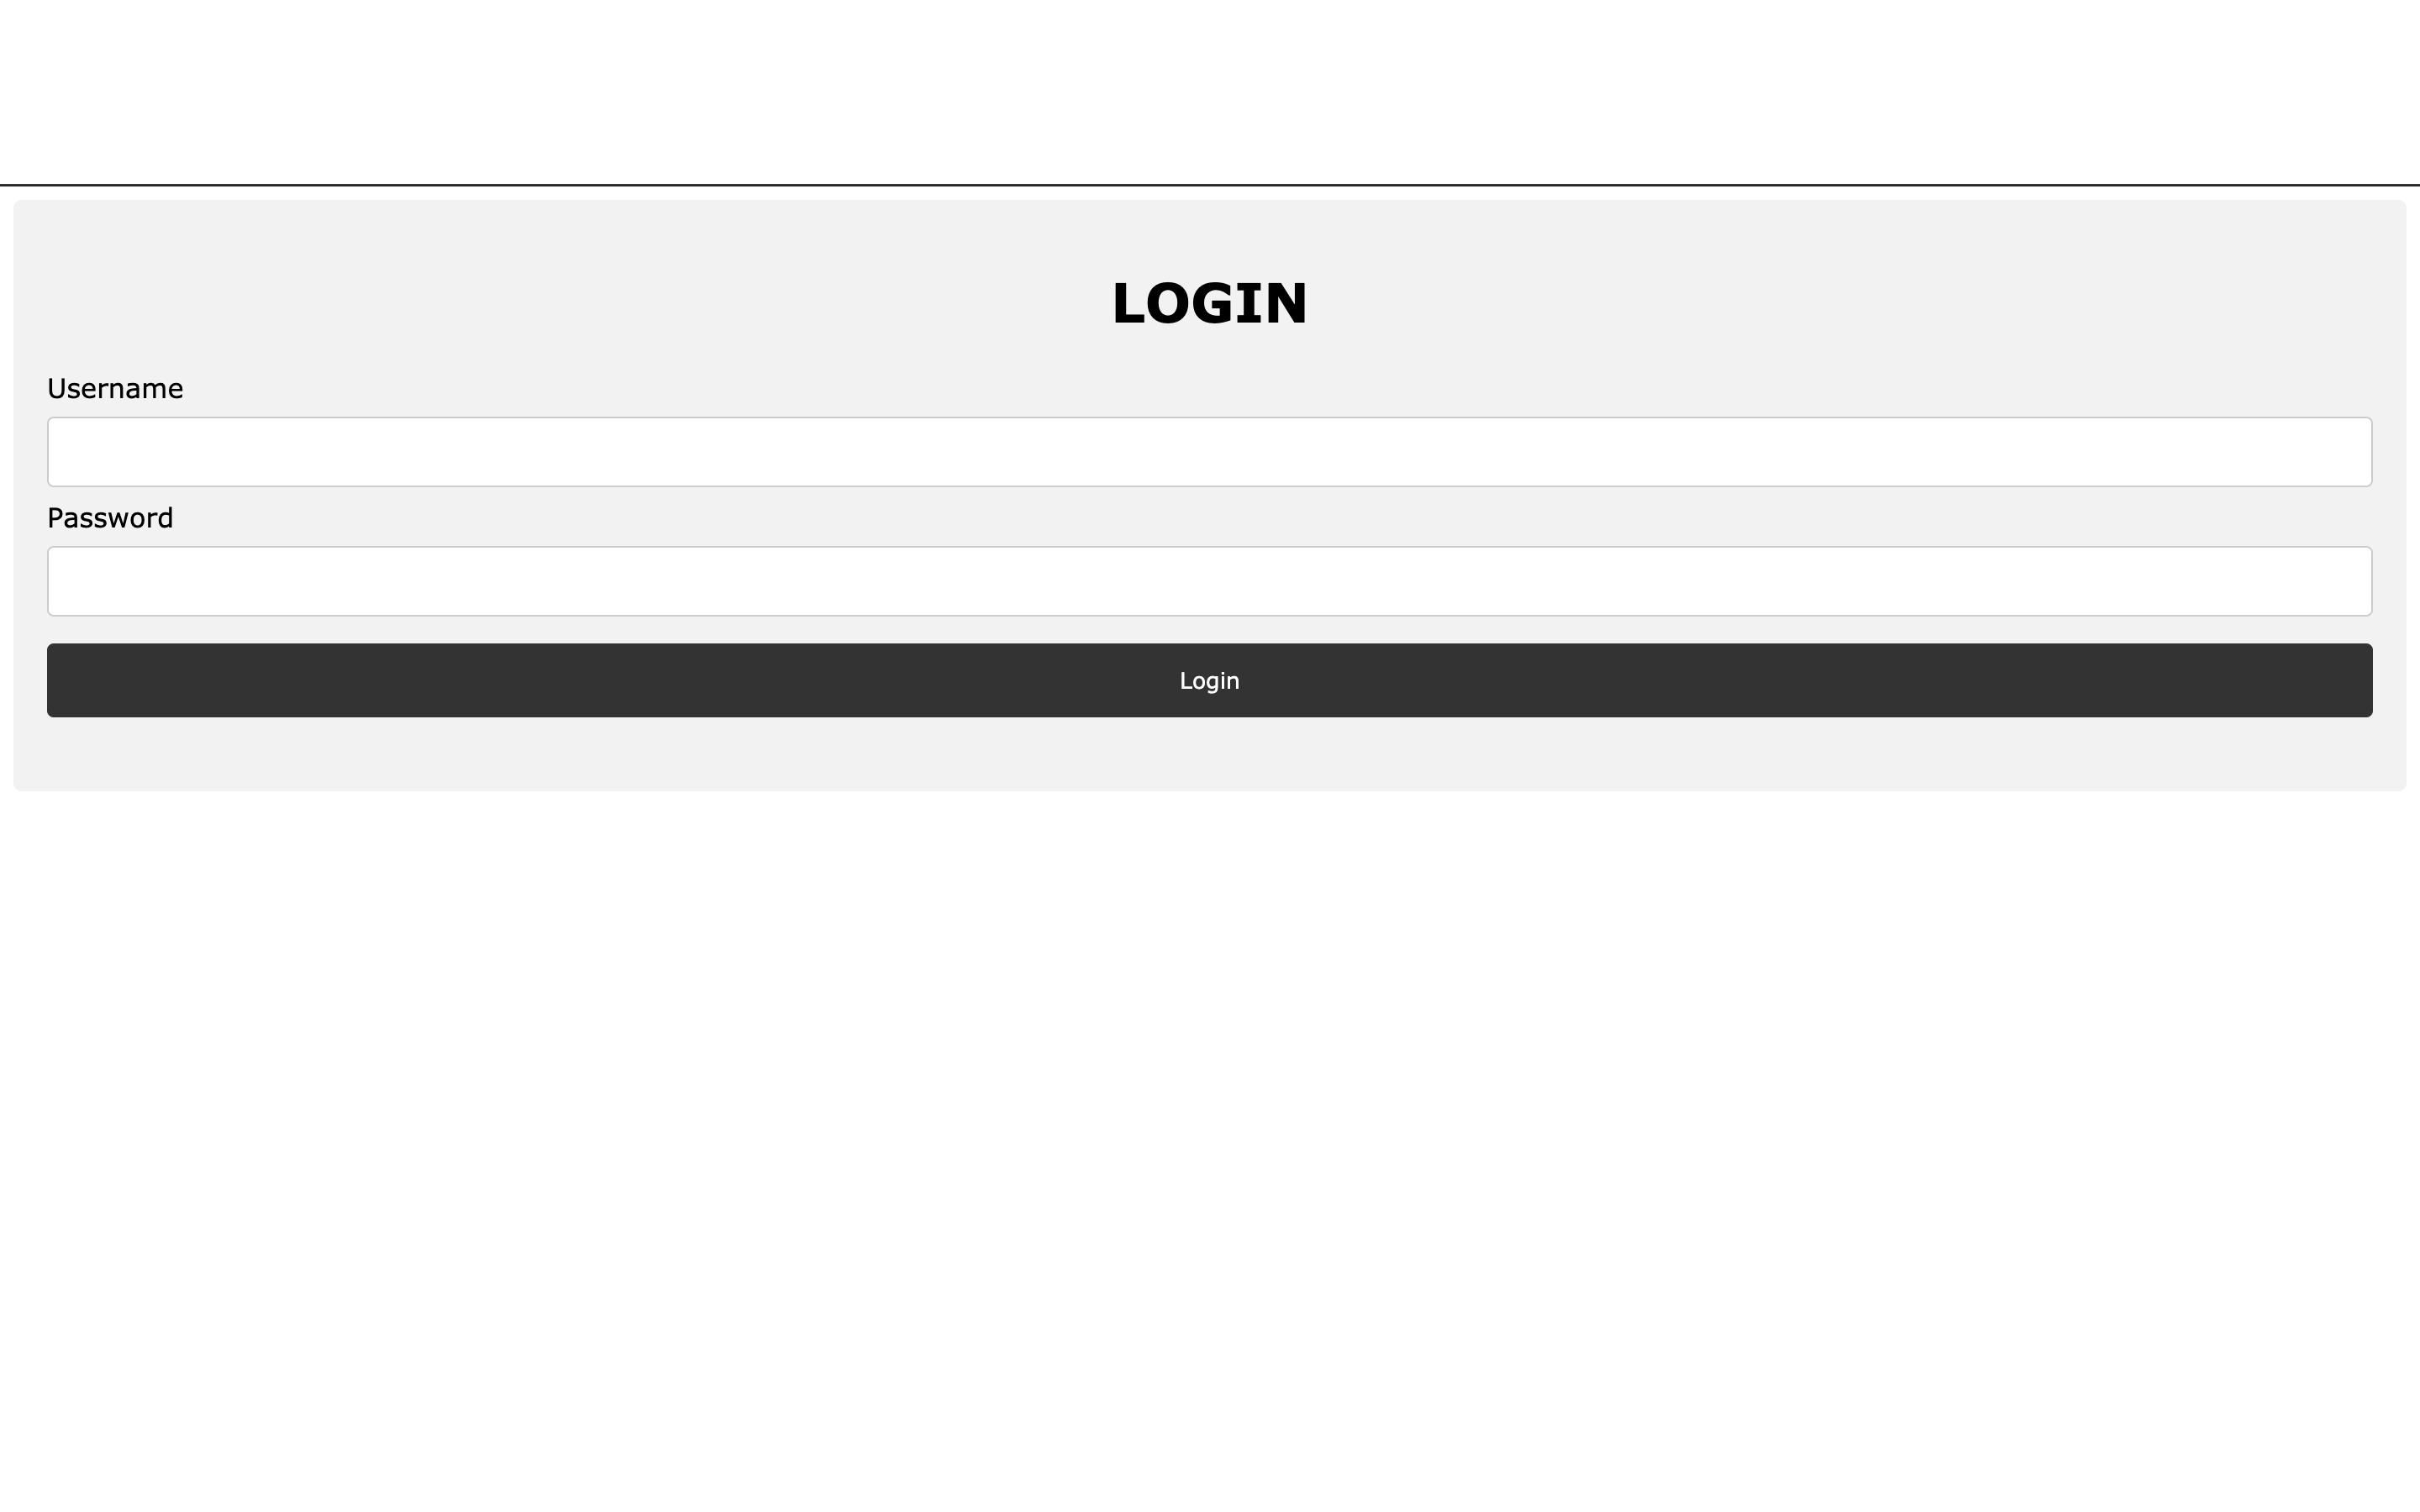
\includegraphics[scale=0.12]{res/images/login.png}
    \caption{Login}
\end{figure}
\subsection{Visualizzazione situazione in real time del magazzino}
\begin{itemize}
    \item Dopo l'autenticazione, tramite il menù selezionare il pulsante "Visualizza mappa";
    \item viene visualizzata la planimetria del magazzino con la relativa legenda e la rappresentazione dei muletti che si spostano;
    \item Per tornare alla pagina iniziale premere sul pulsante "Chiudi".
\end{itemize}

\begin{figure}[H]
    \centering
    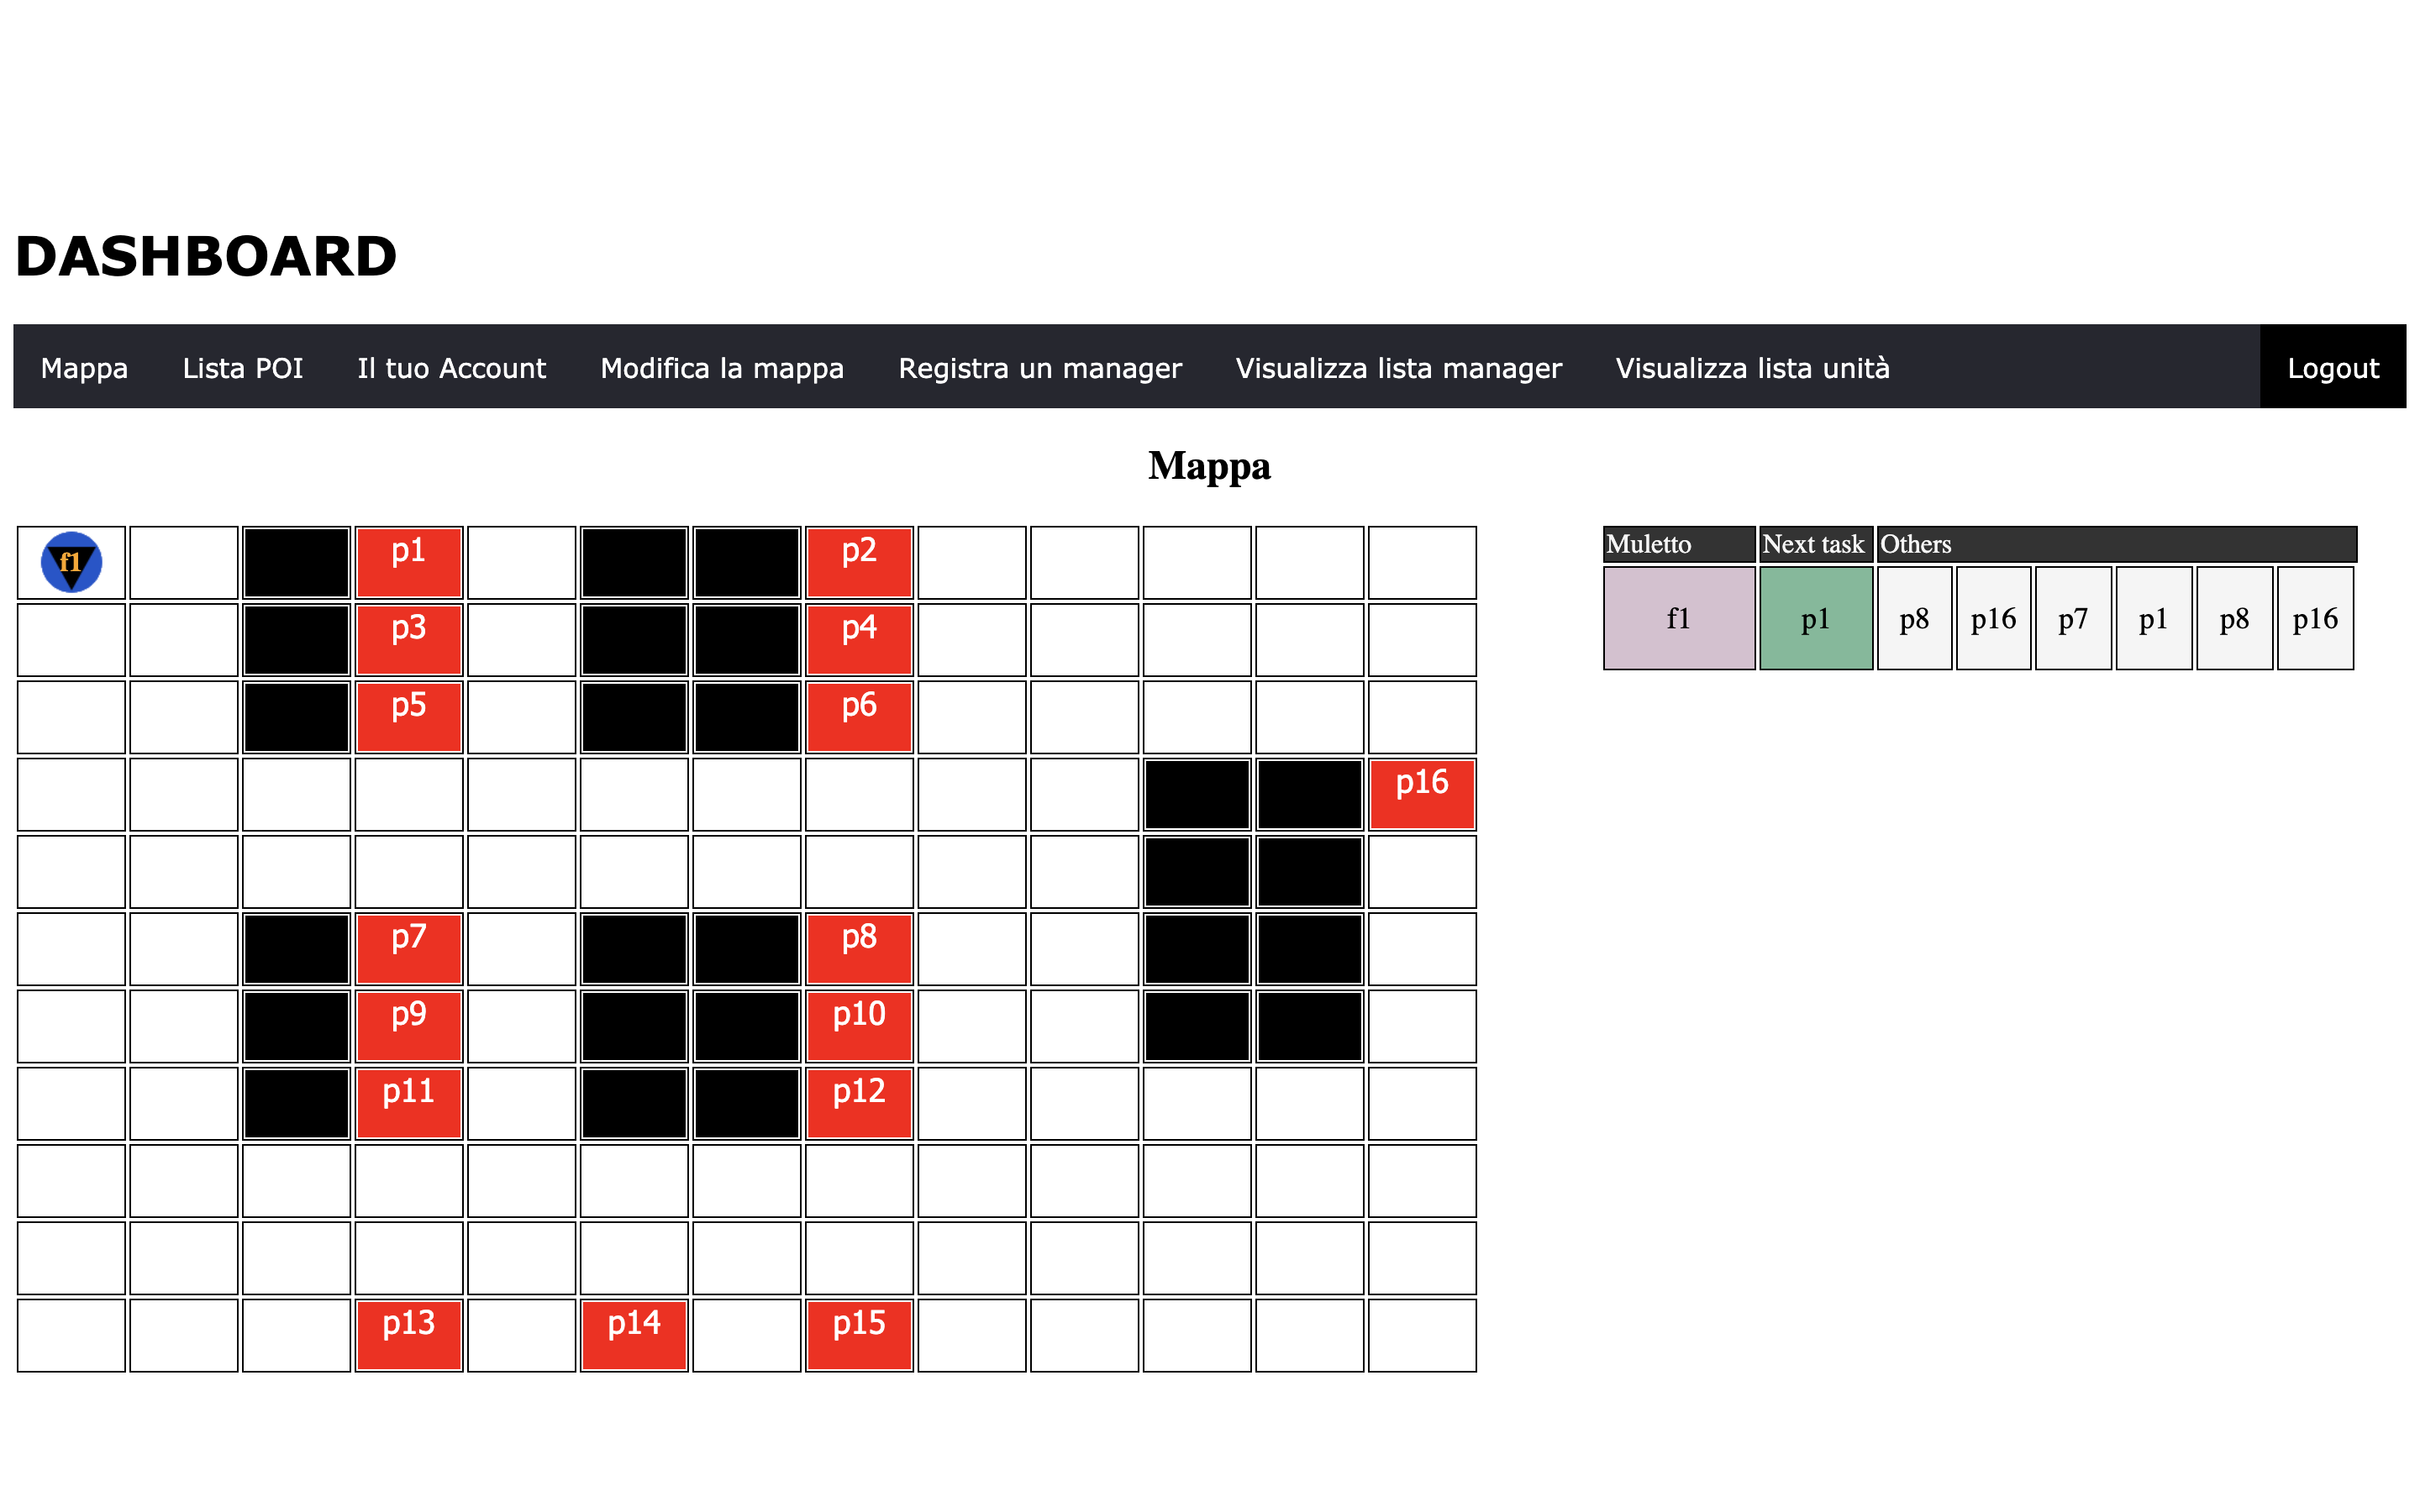
\includegraphics[scale=0.12]{res/images/map_user.png}
    \caption{Schermata guida automatica dell'unità}
\end{figure}

\subsection{Visualizzazione lista completa punti di interesse}
\begin{itemize}
    \item Dopo l'autenticazione, tramite il menù selezionare il pulsante "Visualizza lista POI";
    \item si viene indirizzati alla pagina con l'elenco di tutti i punti di interesse presenti nel magazzino;
    \item Per tornare alla pagina iniziale serve premere sul pulsante "Chiudi".
\end{itemize}

\begin{figure}[H]
    \centering
    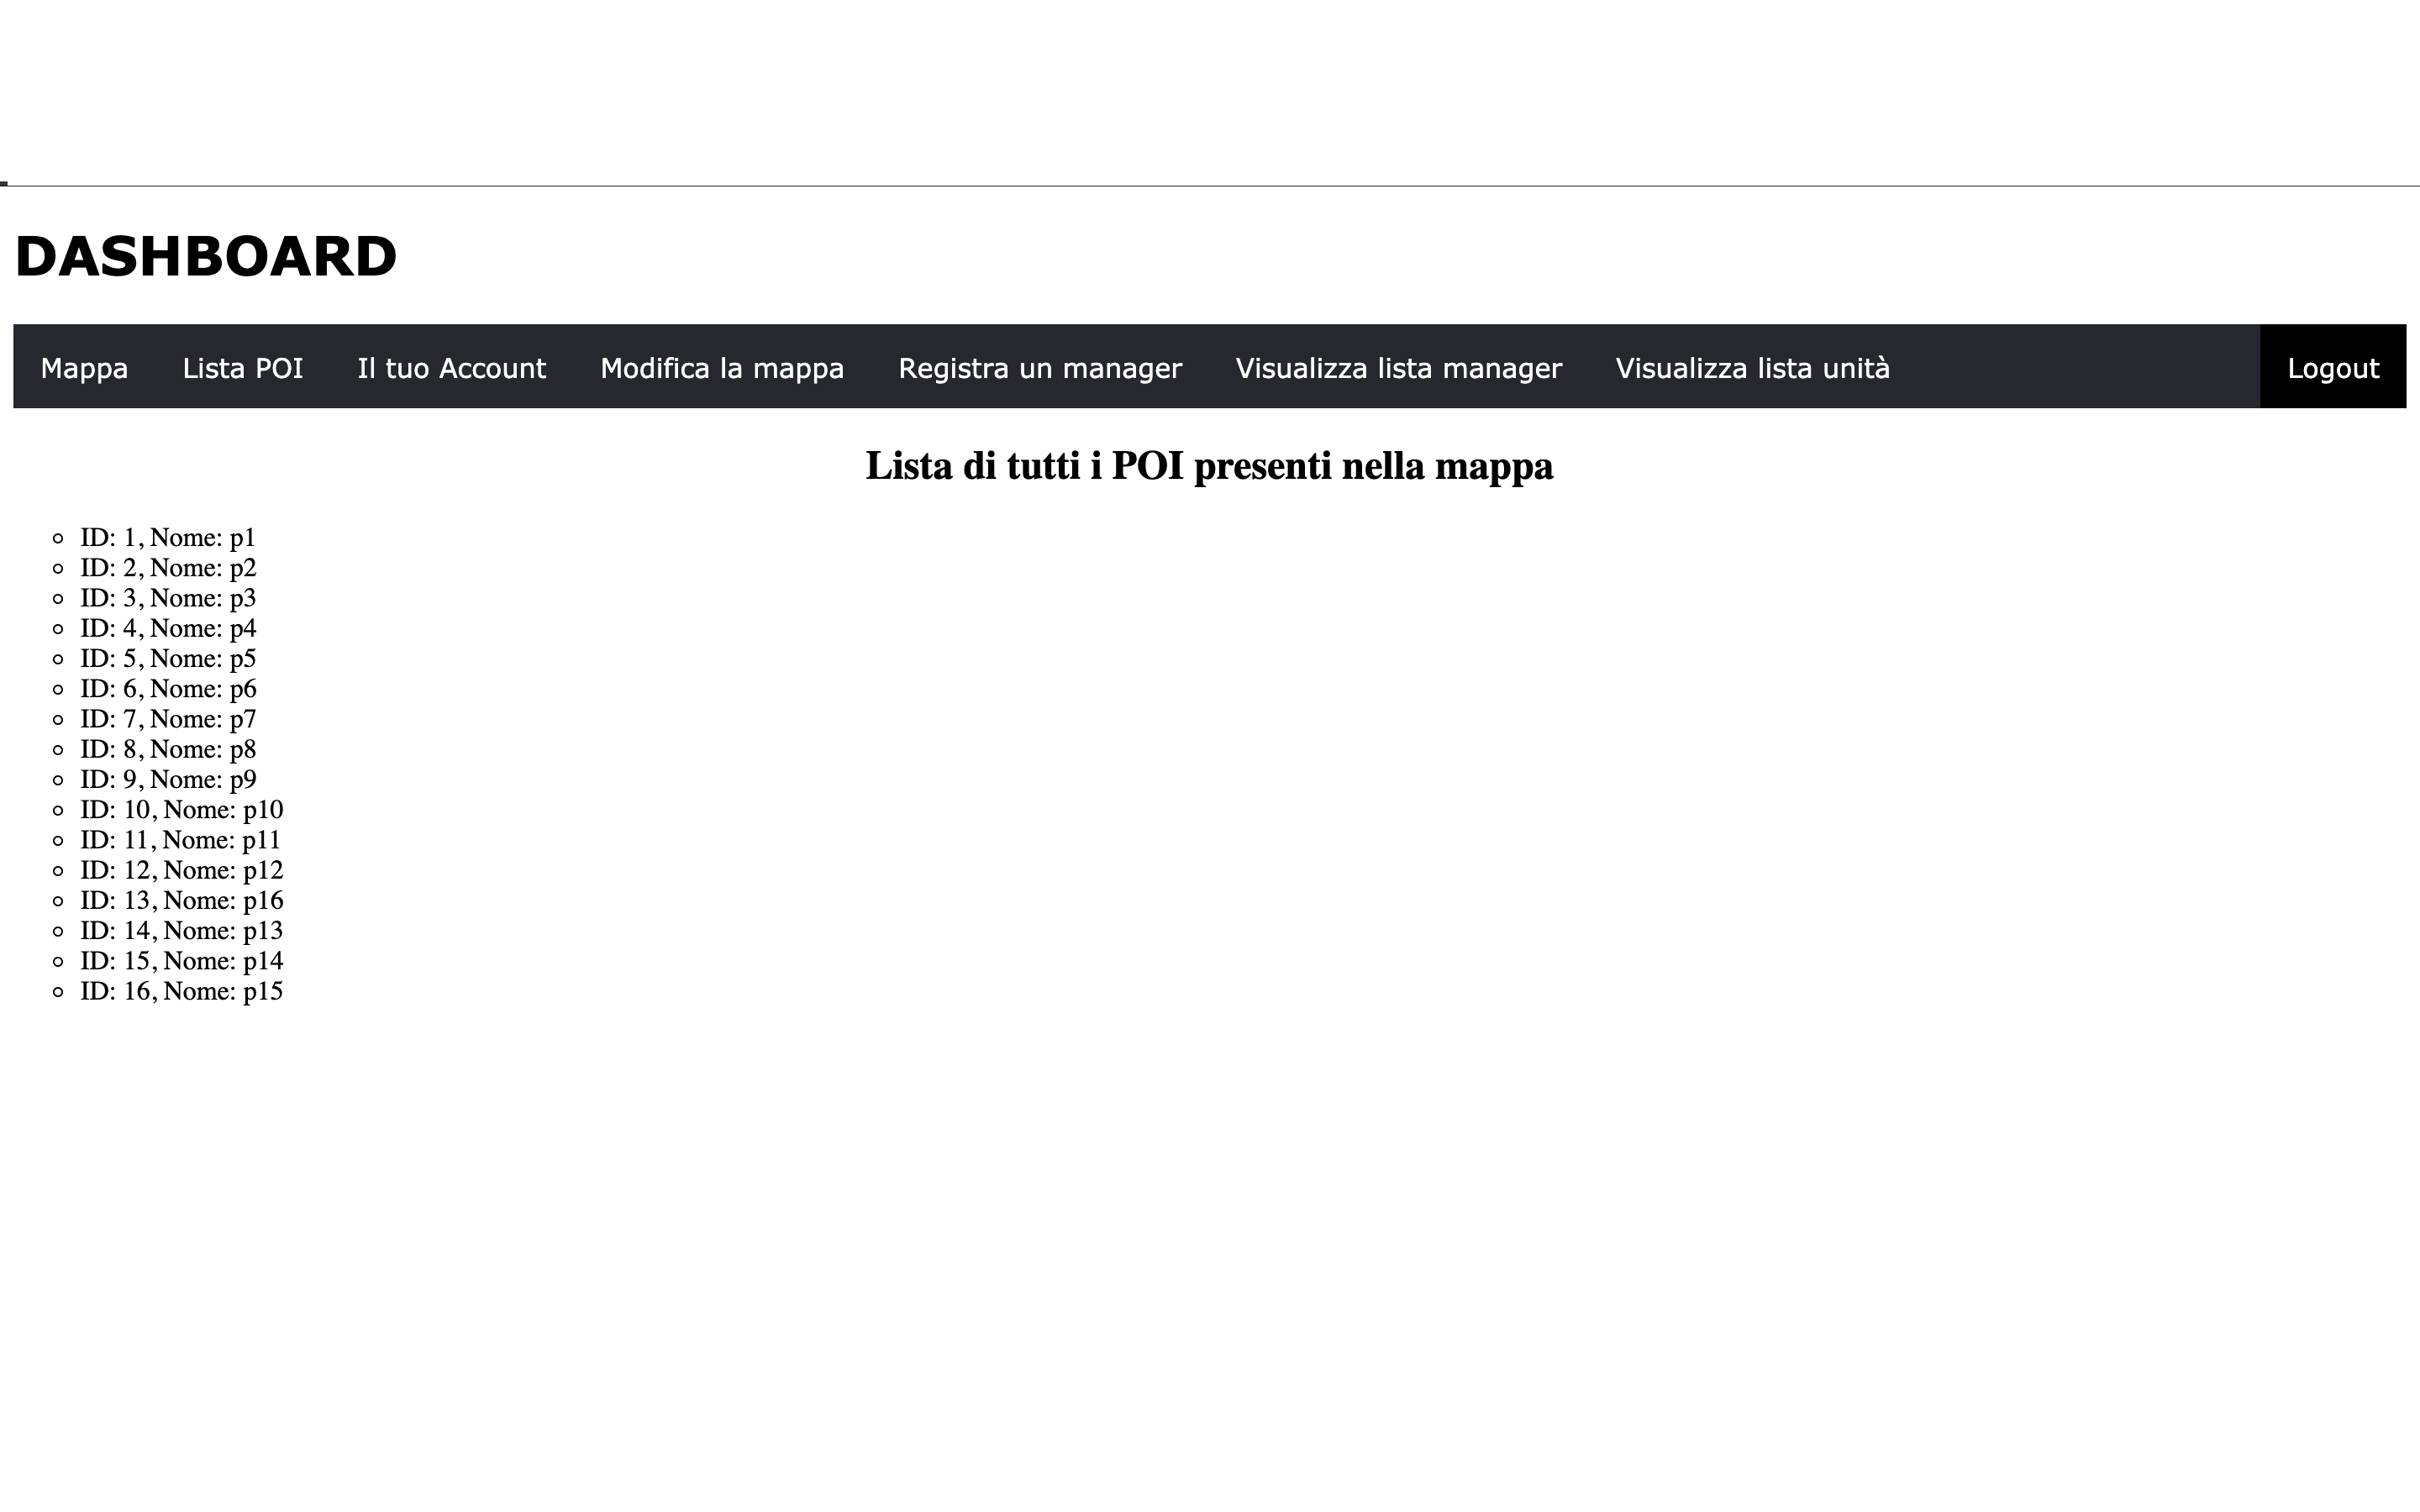
\includegraphics[scale=0.12]{res/images/listpoi_user.png}
    \caption{Schermata guida automatica dell'unità}
\end{figure}

\subsection{Visualizzazione dati del proprio profilo e modifica}
\begin{itemize}
    \item Dopo l'autenticazione, tramite il menù selezionare il pulsante "Visualizza il tuo account";
    \item si viene indirizzati alla pagina con i propri dati utente: nome, cognome, password;
    \item se si desidera modificare alcuni campi, è necessario scrivere nell'apposito form i nuovi dati e premere il pulsante "Conferma";
    \item per tornare alla pagina iniziale serve premere sul pulsante "Chiudi".
\end{itemize}
\begin{figure}[H]
    \centering
    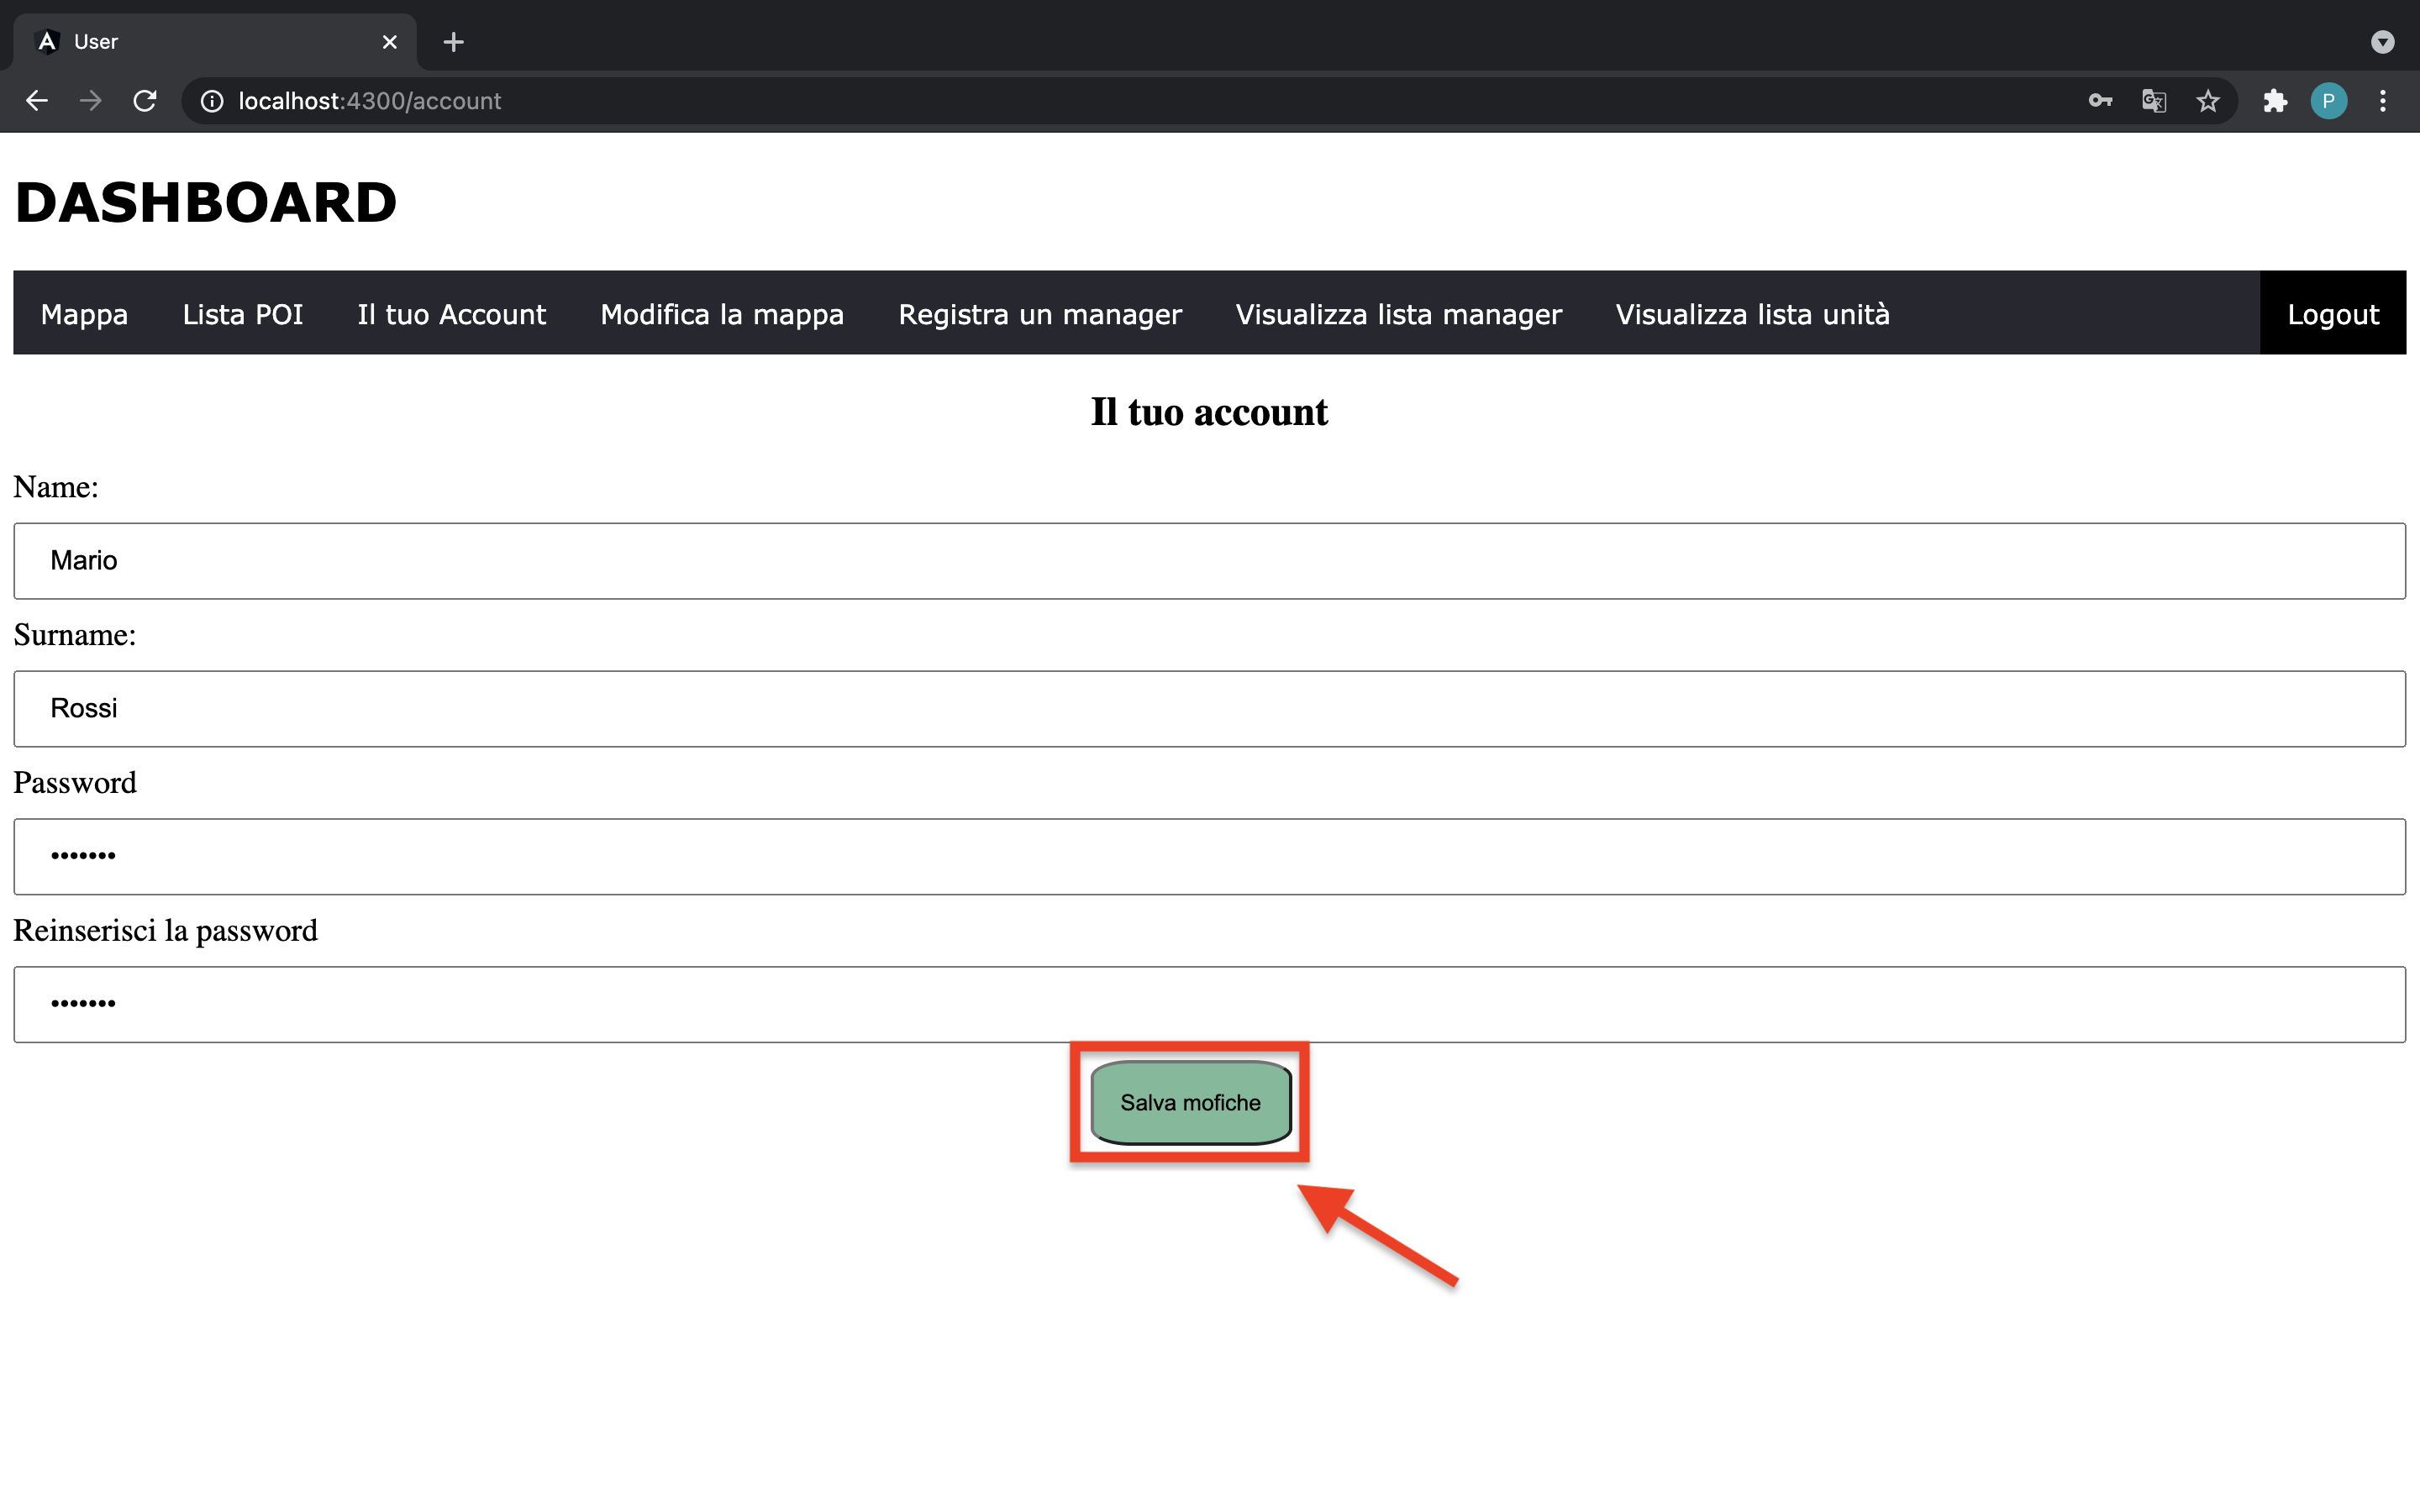
\includegraphics[scale=0.12]{res/images/account_user.png}
    \caption{Schermata guida automatica dell'unità}
\end{figure}

\subsection{Registrazione di un nuovo utente}
\begin{itemize}
    \item Dopo l'autenticazione, tramite il menù selezionare il pulsante "Registra nuovo utente";
    \item si viene indirizzati alla pagina con i campi da compilare: Nome, Cognome;
    \item inserire i dati e premere sul pulsante "Conferma";
    \item viene visualizzato a video la password e il codice identificativo da riferire al nuovo utente per il suo primo accesso;
    \item per tornare alla pagina iniziale serve premere sul pulsante "Chiudi".
\end{itemize}
\begin{figure}[H]
    \centering
    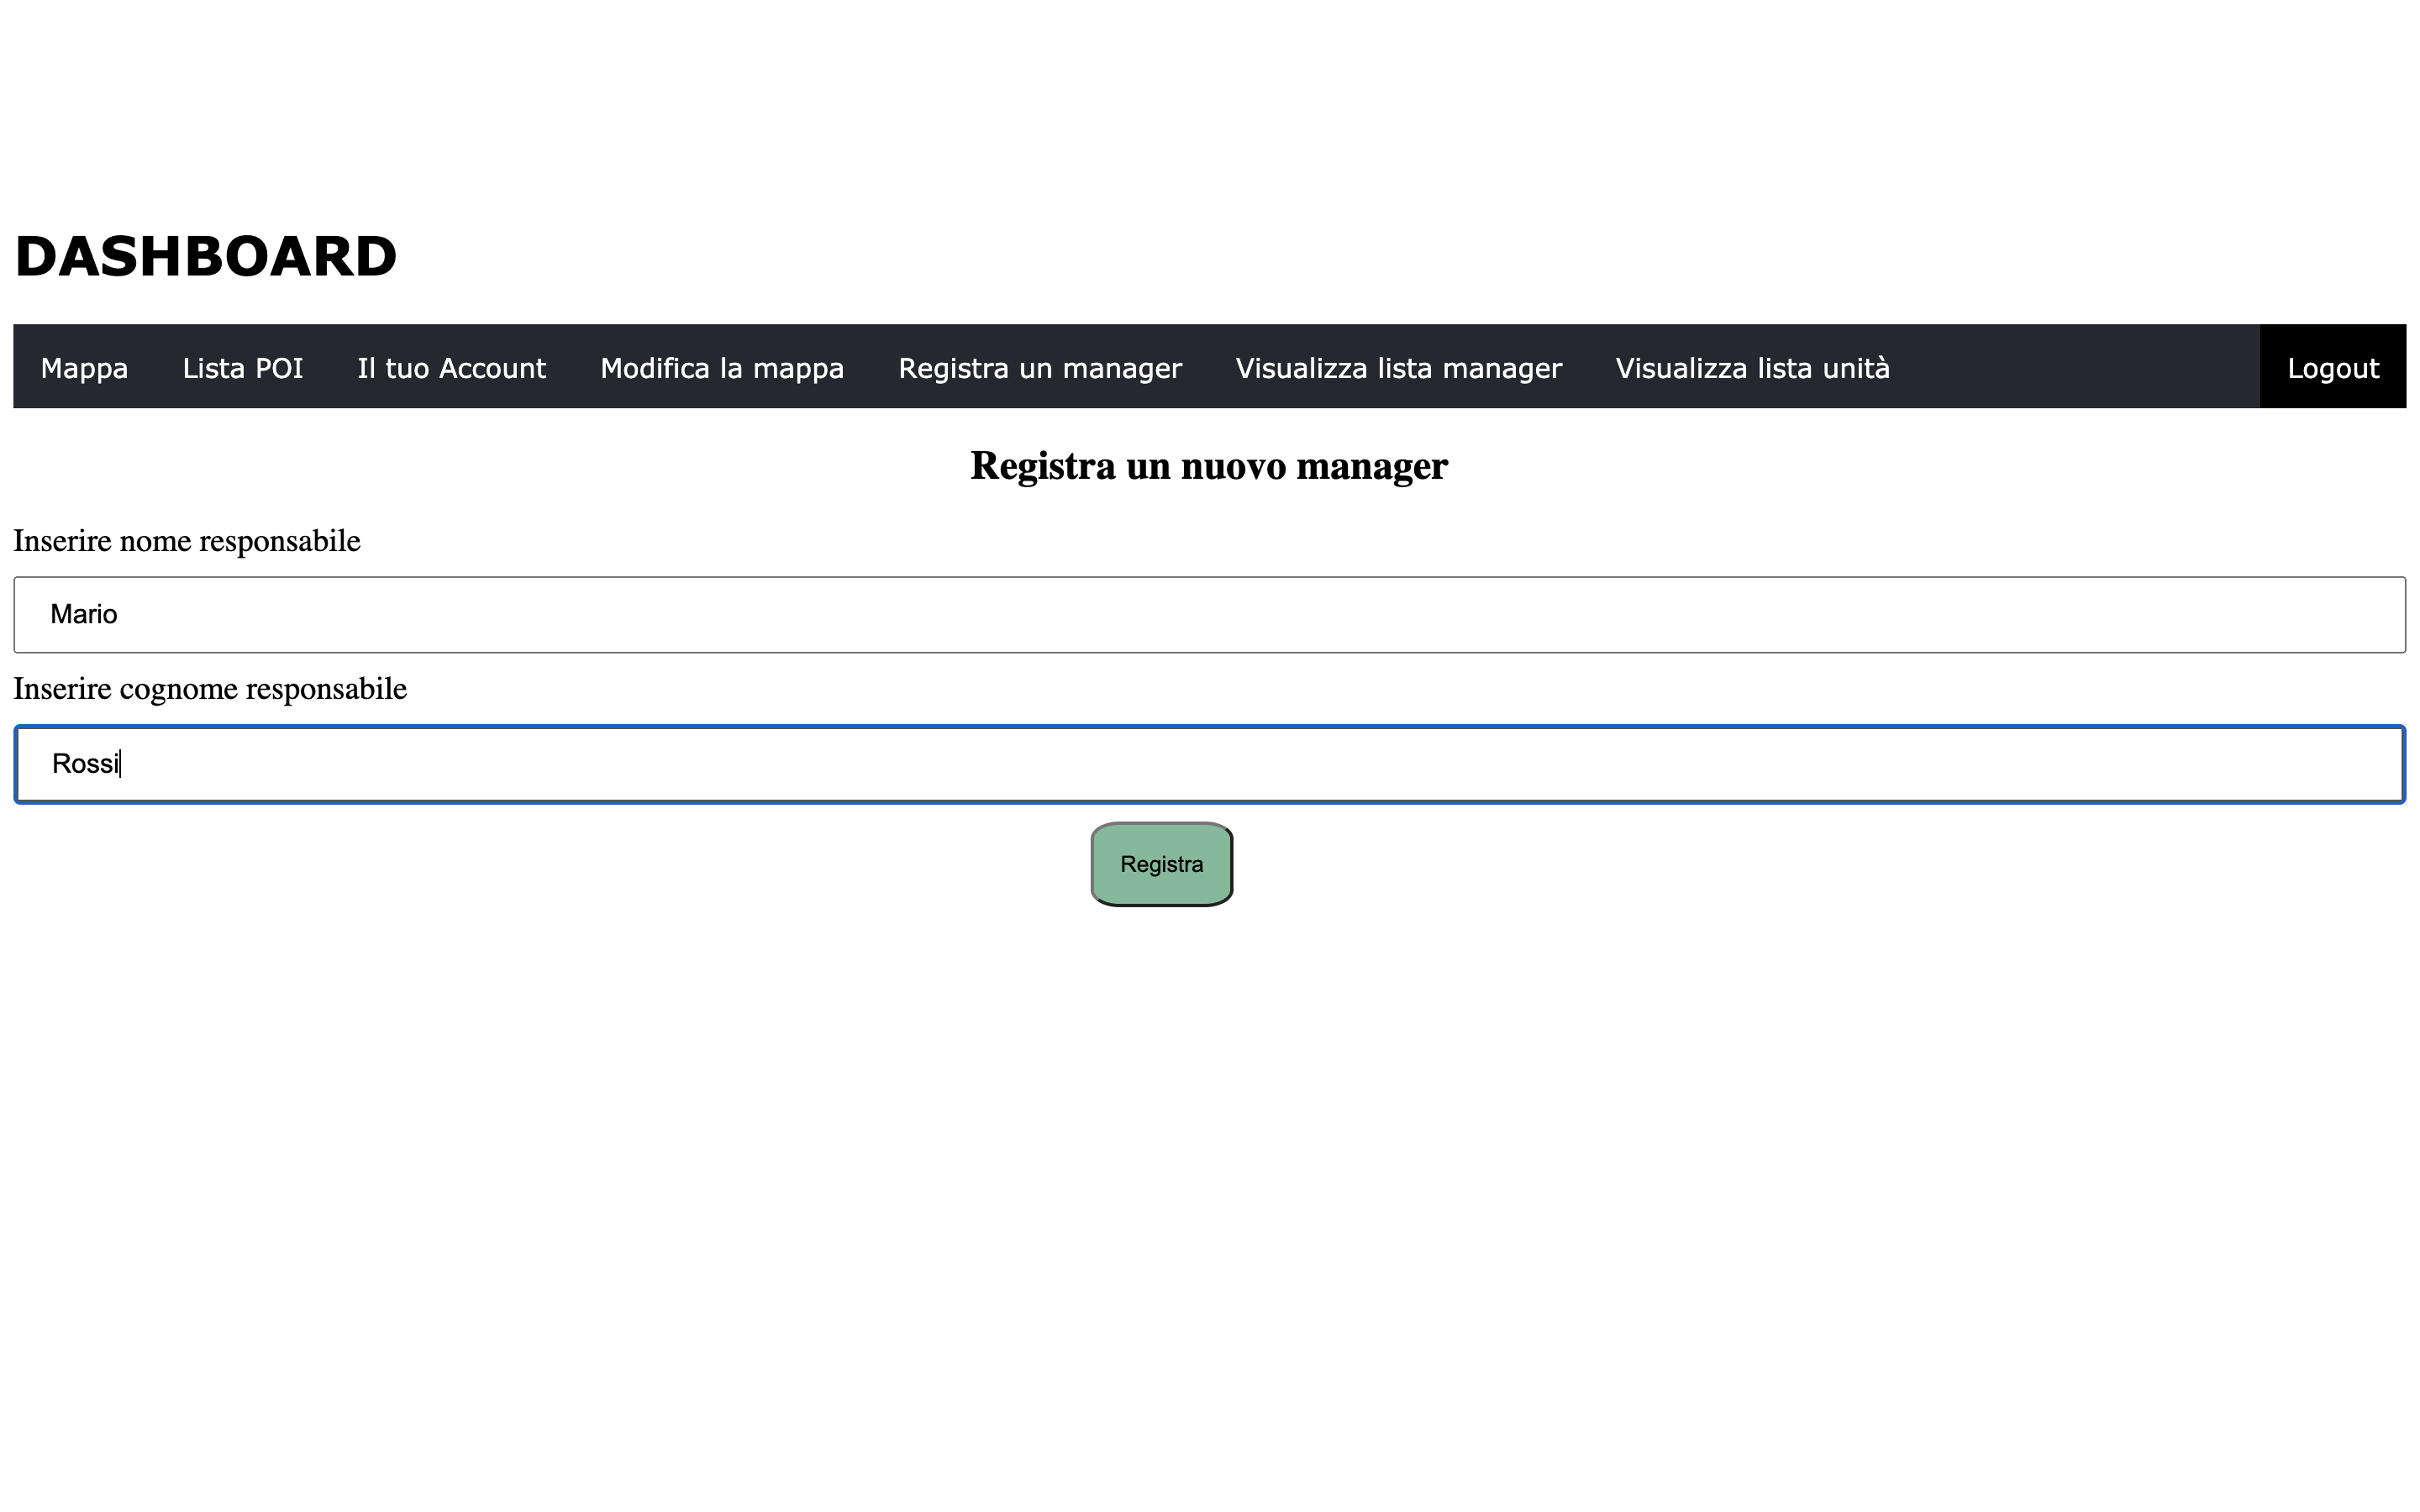
\includegraphics[scale=0.12]{res/images/newmanager_admin.png}
    \caption{Schermata guida automatica dell'unità}
\end{figure}

\begin{figure}[H]
    \centering
    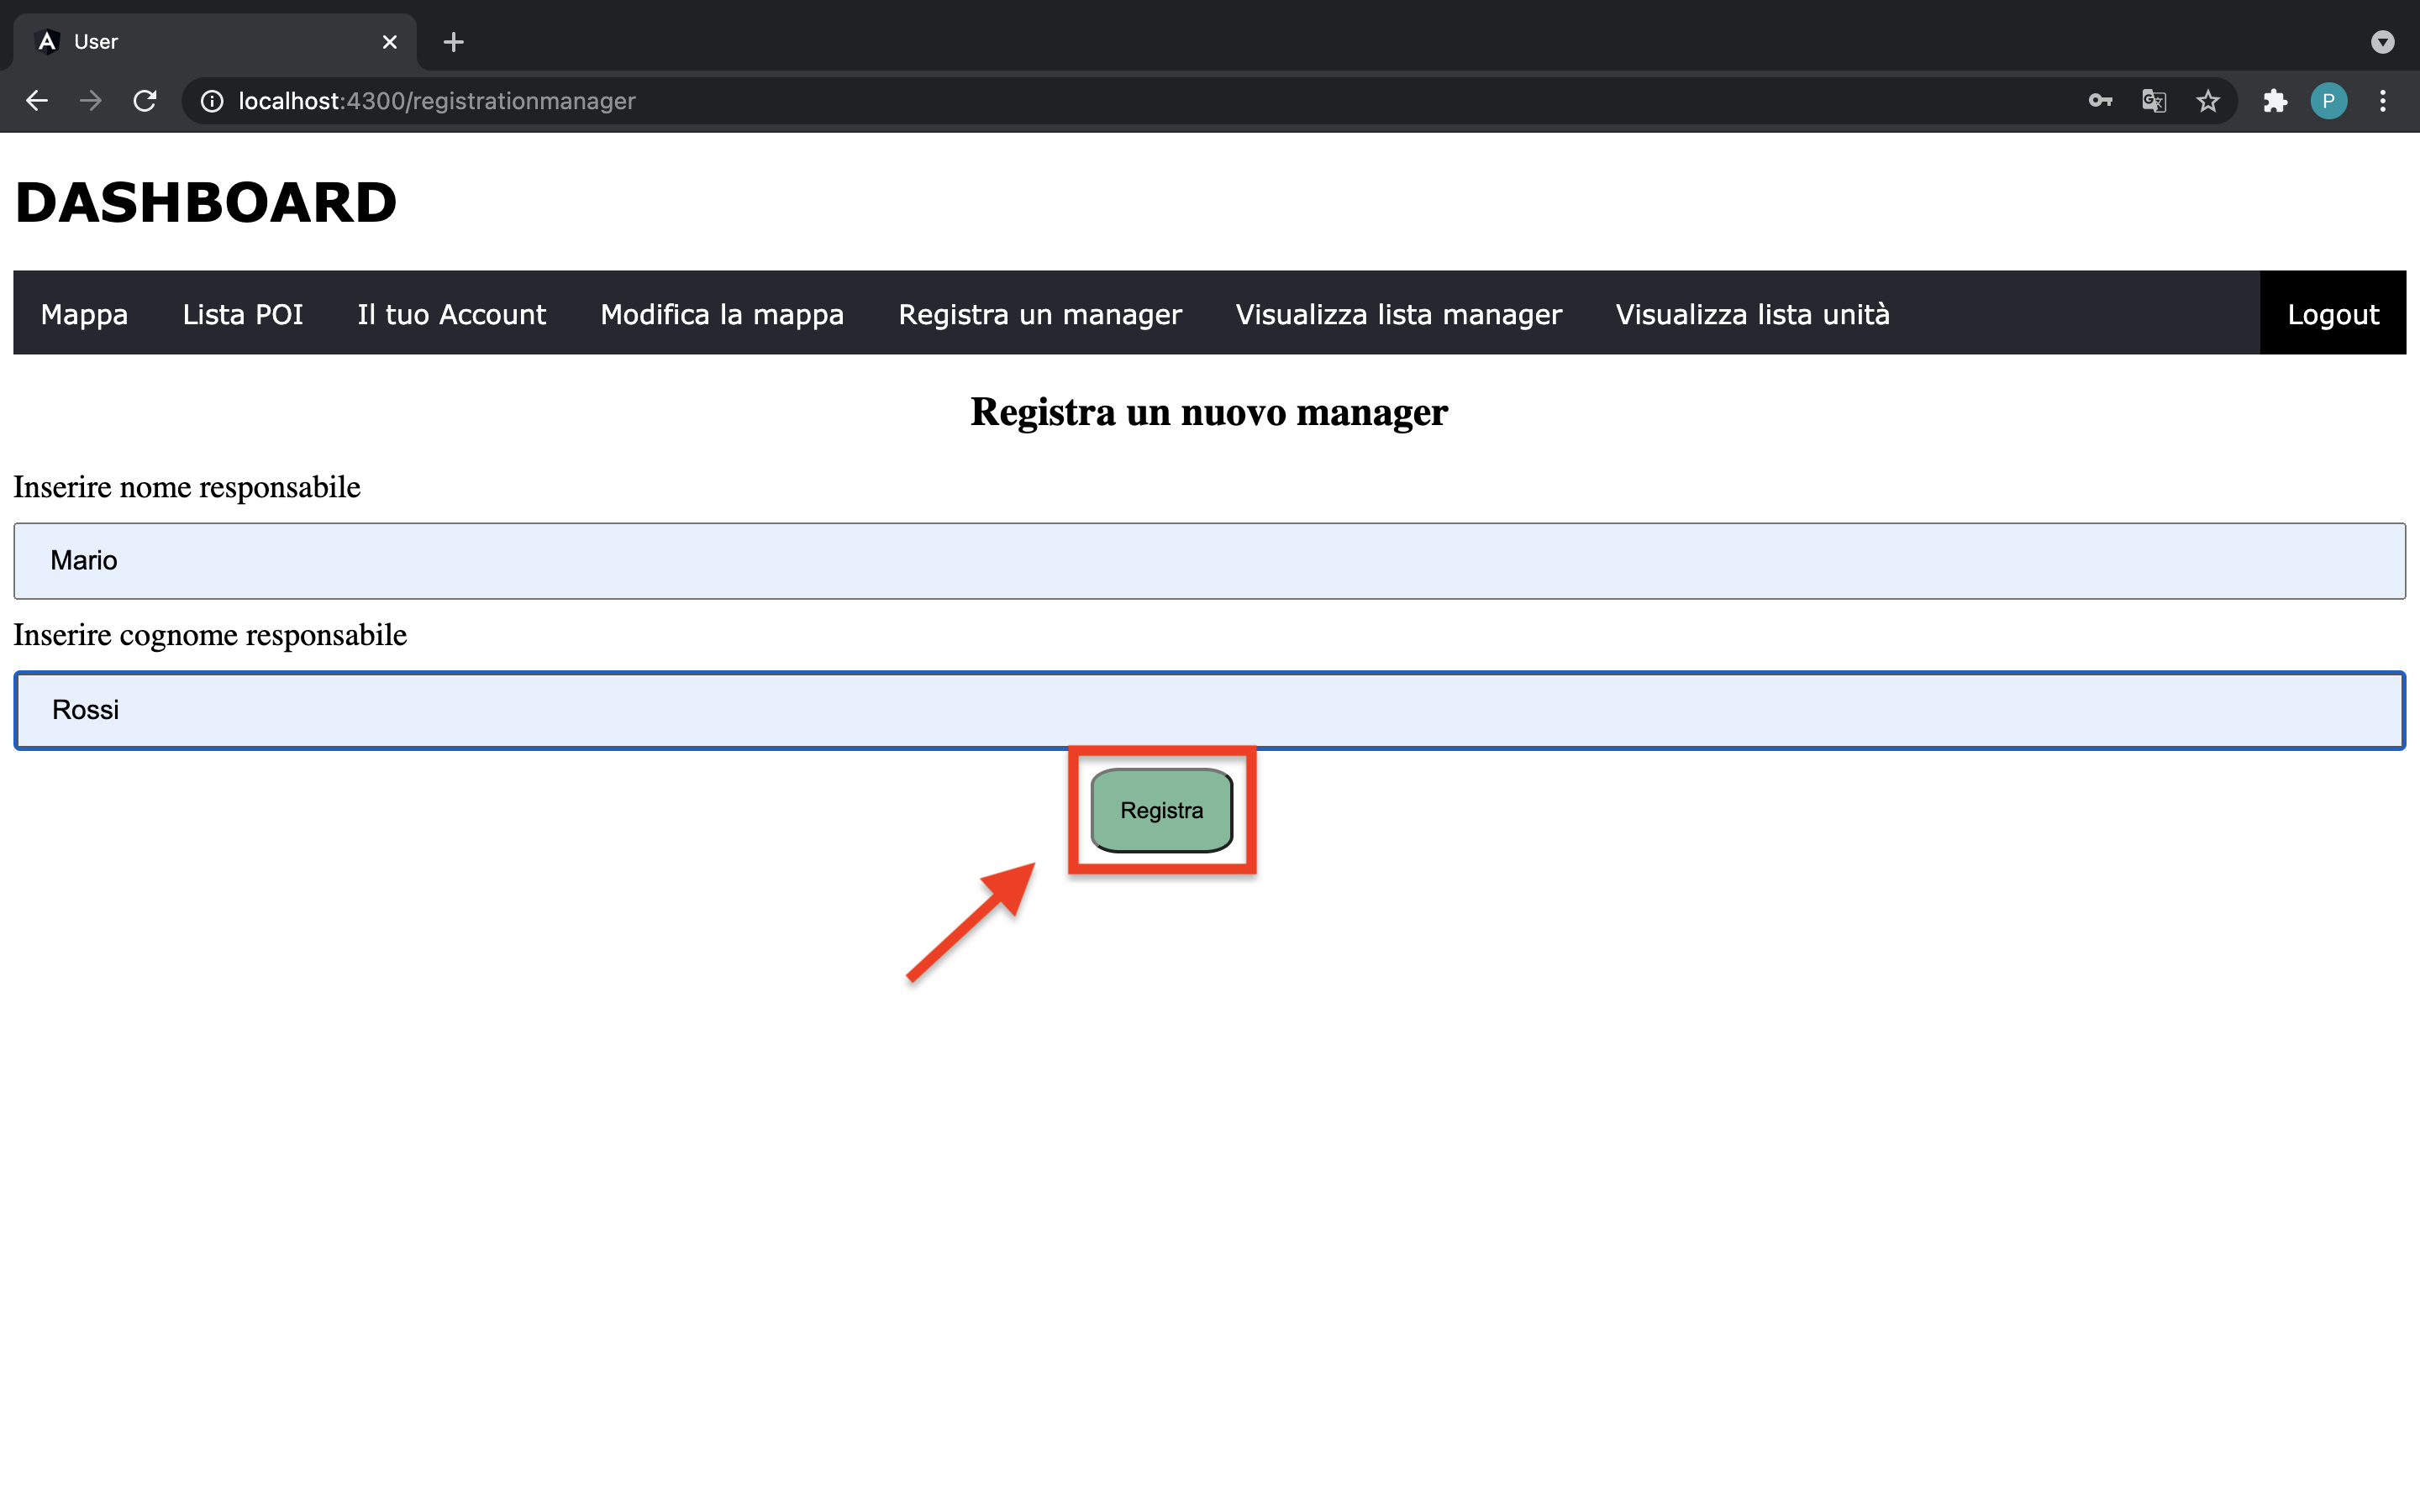
\includegraphics[scale=0.12]{res/images/newmanager_2.png}
    \caption{Schermata guida automatica dell'unità}
\end{figure}

\subsection{Gestione account già presenti}
\begin{itemize}
    \item Dopo l'autenticazione, tramite il menù selezionare il pulsante "Visualizza tutti gli account";
    \item si viene indirizzati alla pagina con la lista di tutti gli account presenti;
    \item di fianco ad ogni account è possibile:
        \begin{itemize}
            \item premere il pulsante "Modifica" per cambiare i dati di questo utente: vengono visualizzati due form "Nome" e "Cognome" in cui scrivere i nuovi dati che verranno poi confermati;
            \item premere il pulsate "Elimina" per cancellare definitivamente un account dal sistema;
            \item premere il pulsante "Reset password" per cambiare la password di un utente in caso di smarrimento;
        \end{itemize}
    \item per tornare alla pagina iniziale serve premere sul pulsante "Chiudi".
\end{itemize}

\begin{figure}[H]
    \centering
    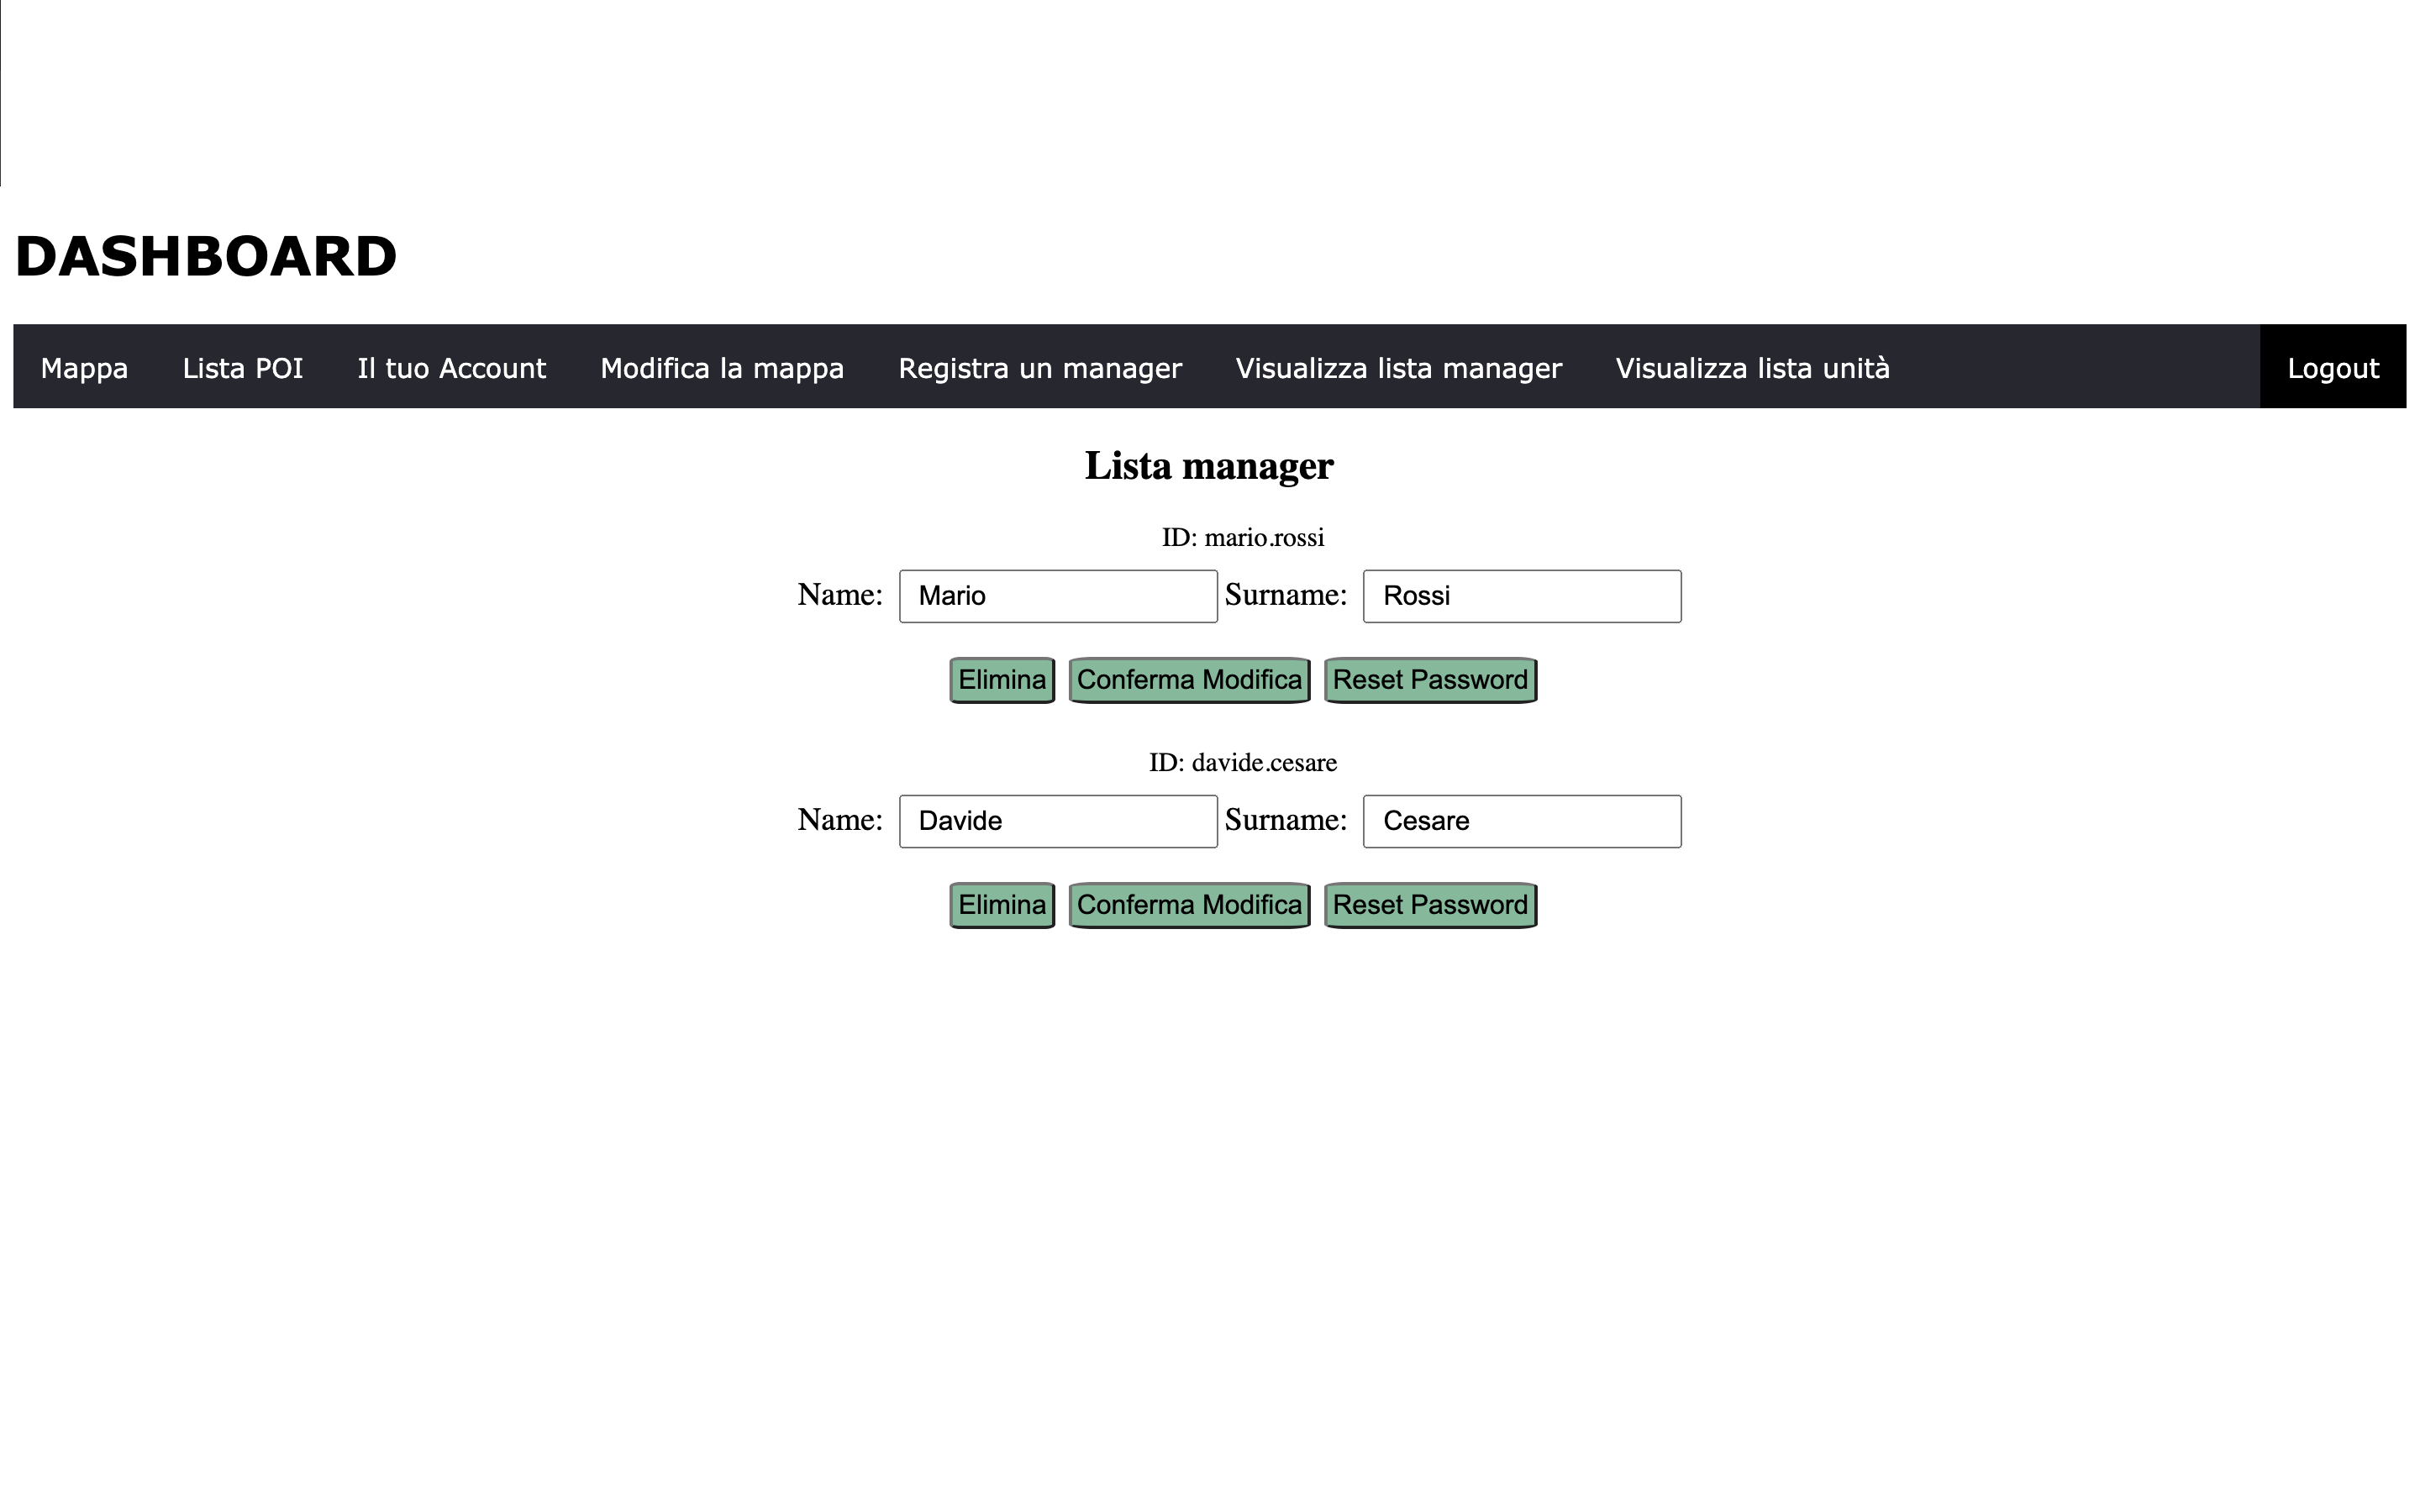
\includegraphics[scale=0.12]{res/images/listmanager_admin.png}
    \caption{Schermata guida automatica dell'unità}
\end{figure}

\subsection{Modifica mappa del magazzino}
\begin{itemize}
    \item Dopo l'autenticazione, tramite il menù selezionare il pulsante "Modifica mappa";
    \item si viene indirizzati alla pagina con la rappresentazione della mappa;
    \item è possibile intraprendere le seguenti operazioni:
        \begin{itemize}
            \item aggiungere una riga: \\premere sul pulsante "Aggiungi riga" per ampliare la planimetria di una riga;
            \item eliminare una riga: \\premere sul pulsante "Rimuovi riga" per diminuire la planimetria di una riga;
            \item aggiungere una colonna: \\premere sul pulsante "Aggiungi colonna" per ampliare la planimetria di una colonna;
            \item eliminare una colonna: \\premere sul pulsante "Rimuovi colonna" per diminuire la planimetria di una colonna;
            \item cambiare il tipo di cella: \\premere sulla cella nella mappa che si intende modificare. Verrà allora visualizzata un'interfaccia con i colori possibili (bianco: zona transitabile, nero: zona non transitabile, frecce: sensi unici, rosso: POI). Nel caso di POI è possibile scrivere l'identificativo. \\Una volta scelto premere sul tasto "Conferma".
        \end{itemize}
    \item quando si è soddisfatti delle modifiche premere sul pulsante "Conferma";
    \item per tornare alla pagina iniziale serve premere sul pulsante "Chiudi".
\end{itemize}
\begin{figure}[H]
    \centering
    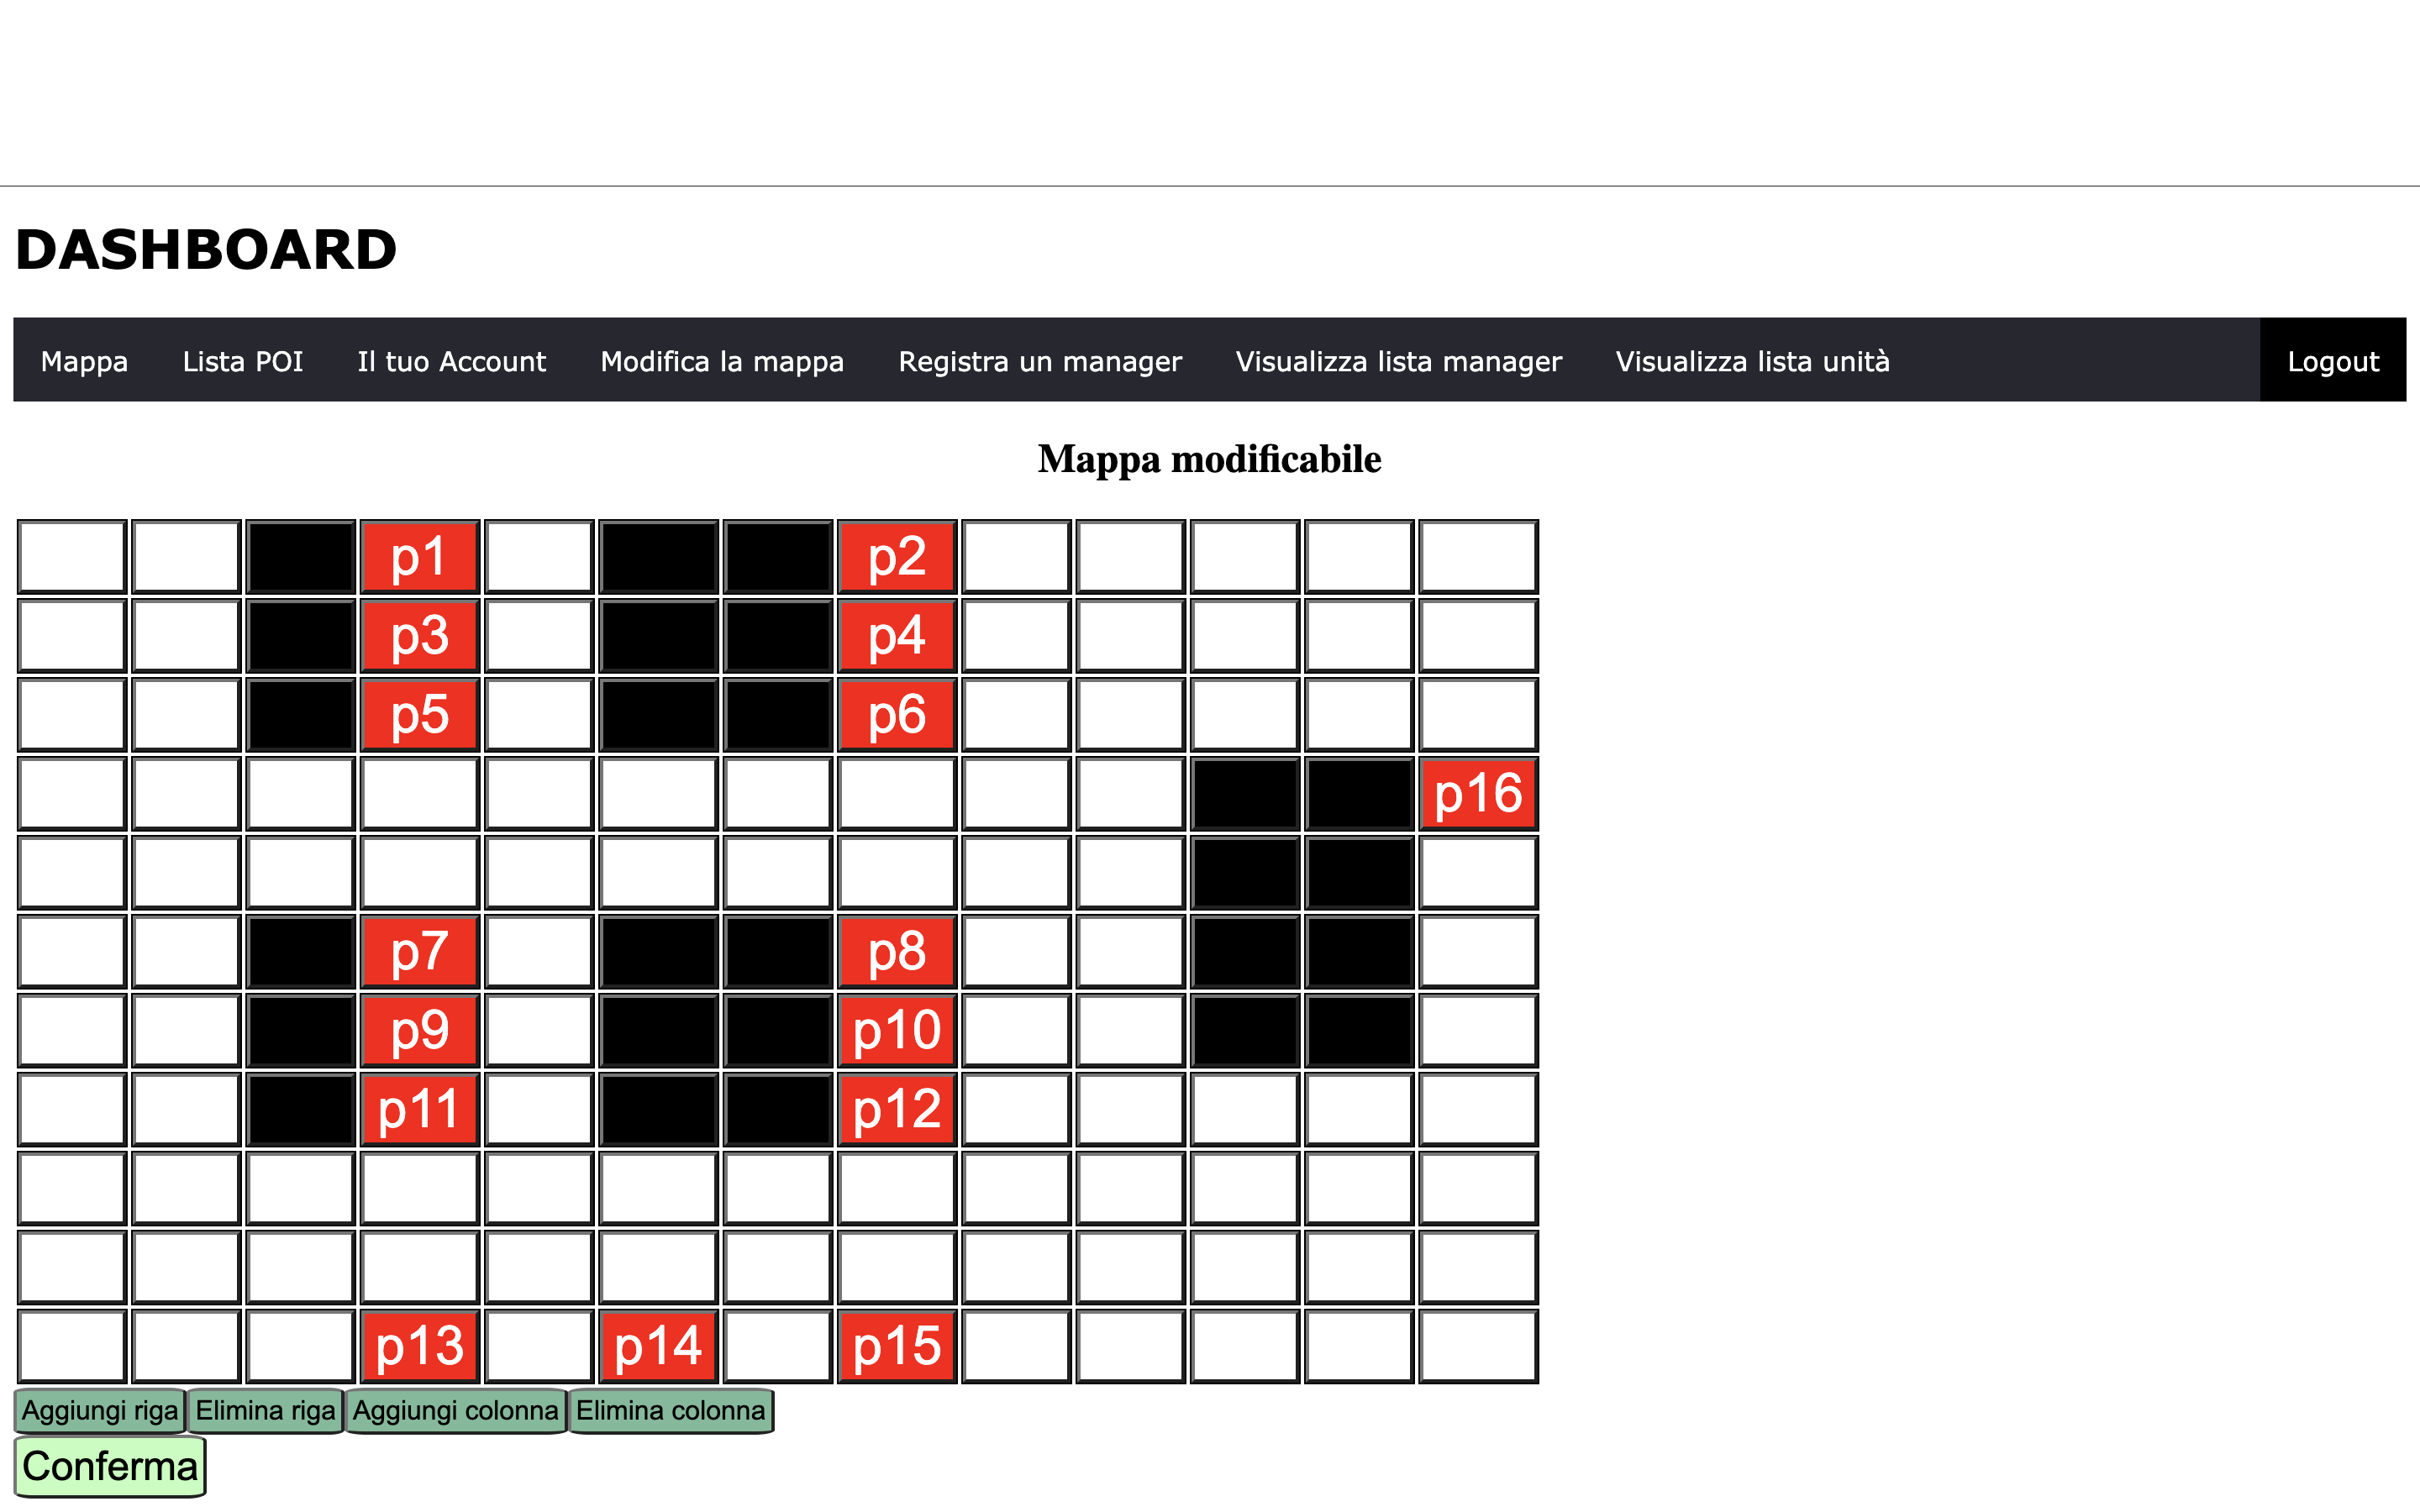
\includegraphics[scale=0.12]{res/images/managemap_admni1.png}
    \caption{Schermata guida automatica dell'unità}
\end{figure}

\subsection{Gestione unità}
\begin{itemize}
\item Dopo l'autenticazione, tramite il menù selezionare il pulsante "Gestione unità"; è possibile effettuare le seguenti operazioni:
    \item aggiungere una nuova unità: \\premere il pulsante "Aggiungi unità" e inserire il codice identificativo nel form;
    \item eliminare un'unità presente: 
    \begin{itemize}
        \item premere il pulsante "Elimina unità";
        \item viene visualizzata la lista di tutte le unità e selezionare quella interessata;
        \item premere il tasto apposito per confermare l'operazione;
    \end{itemize}
    \item per tornare alla pagina iniziale serve premere sul pulsante "Chiudi".
\end{itemize}
\begin{figure}[H]
    \centering
    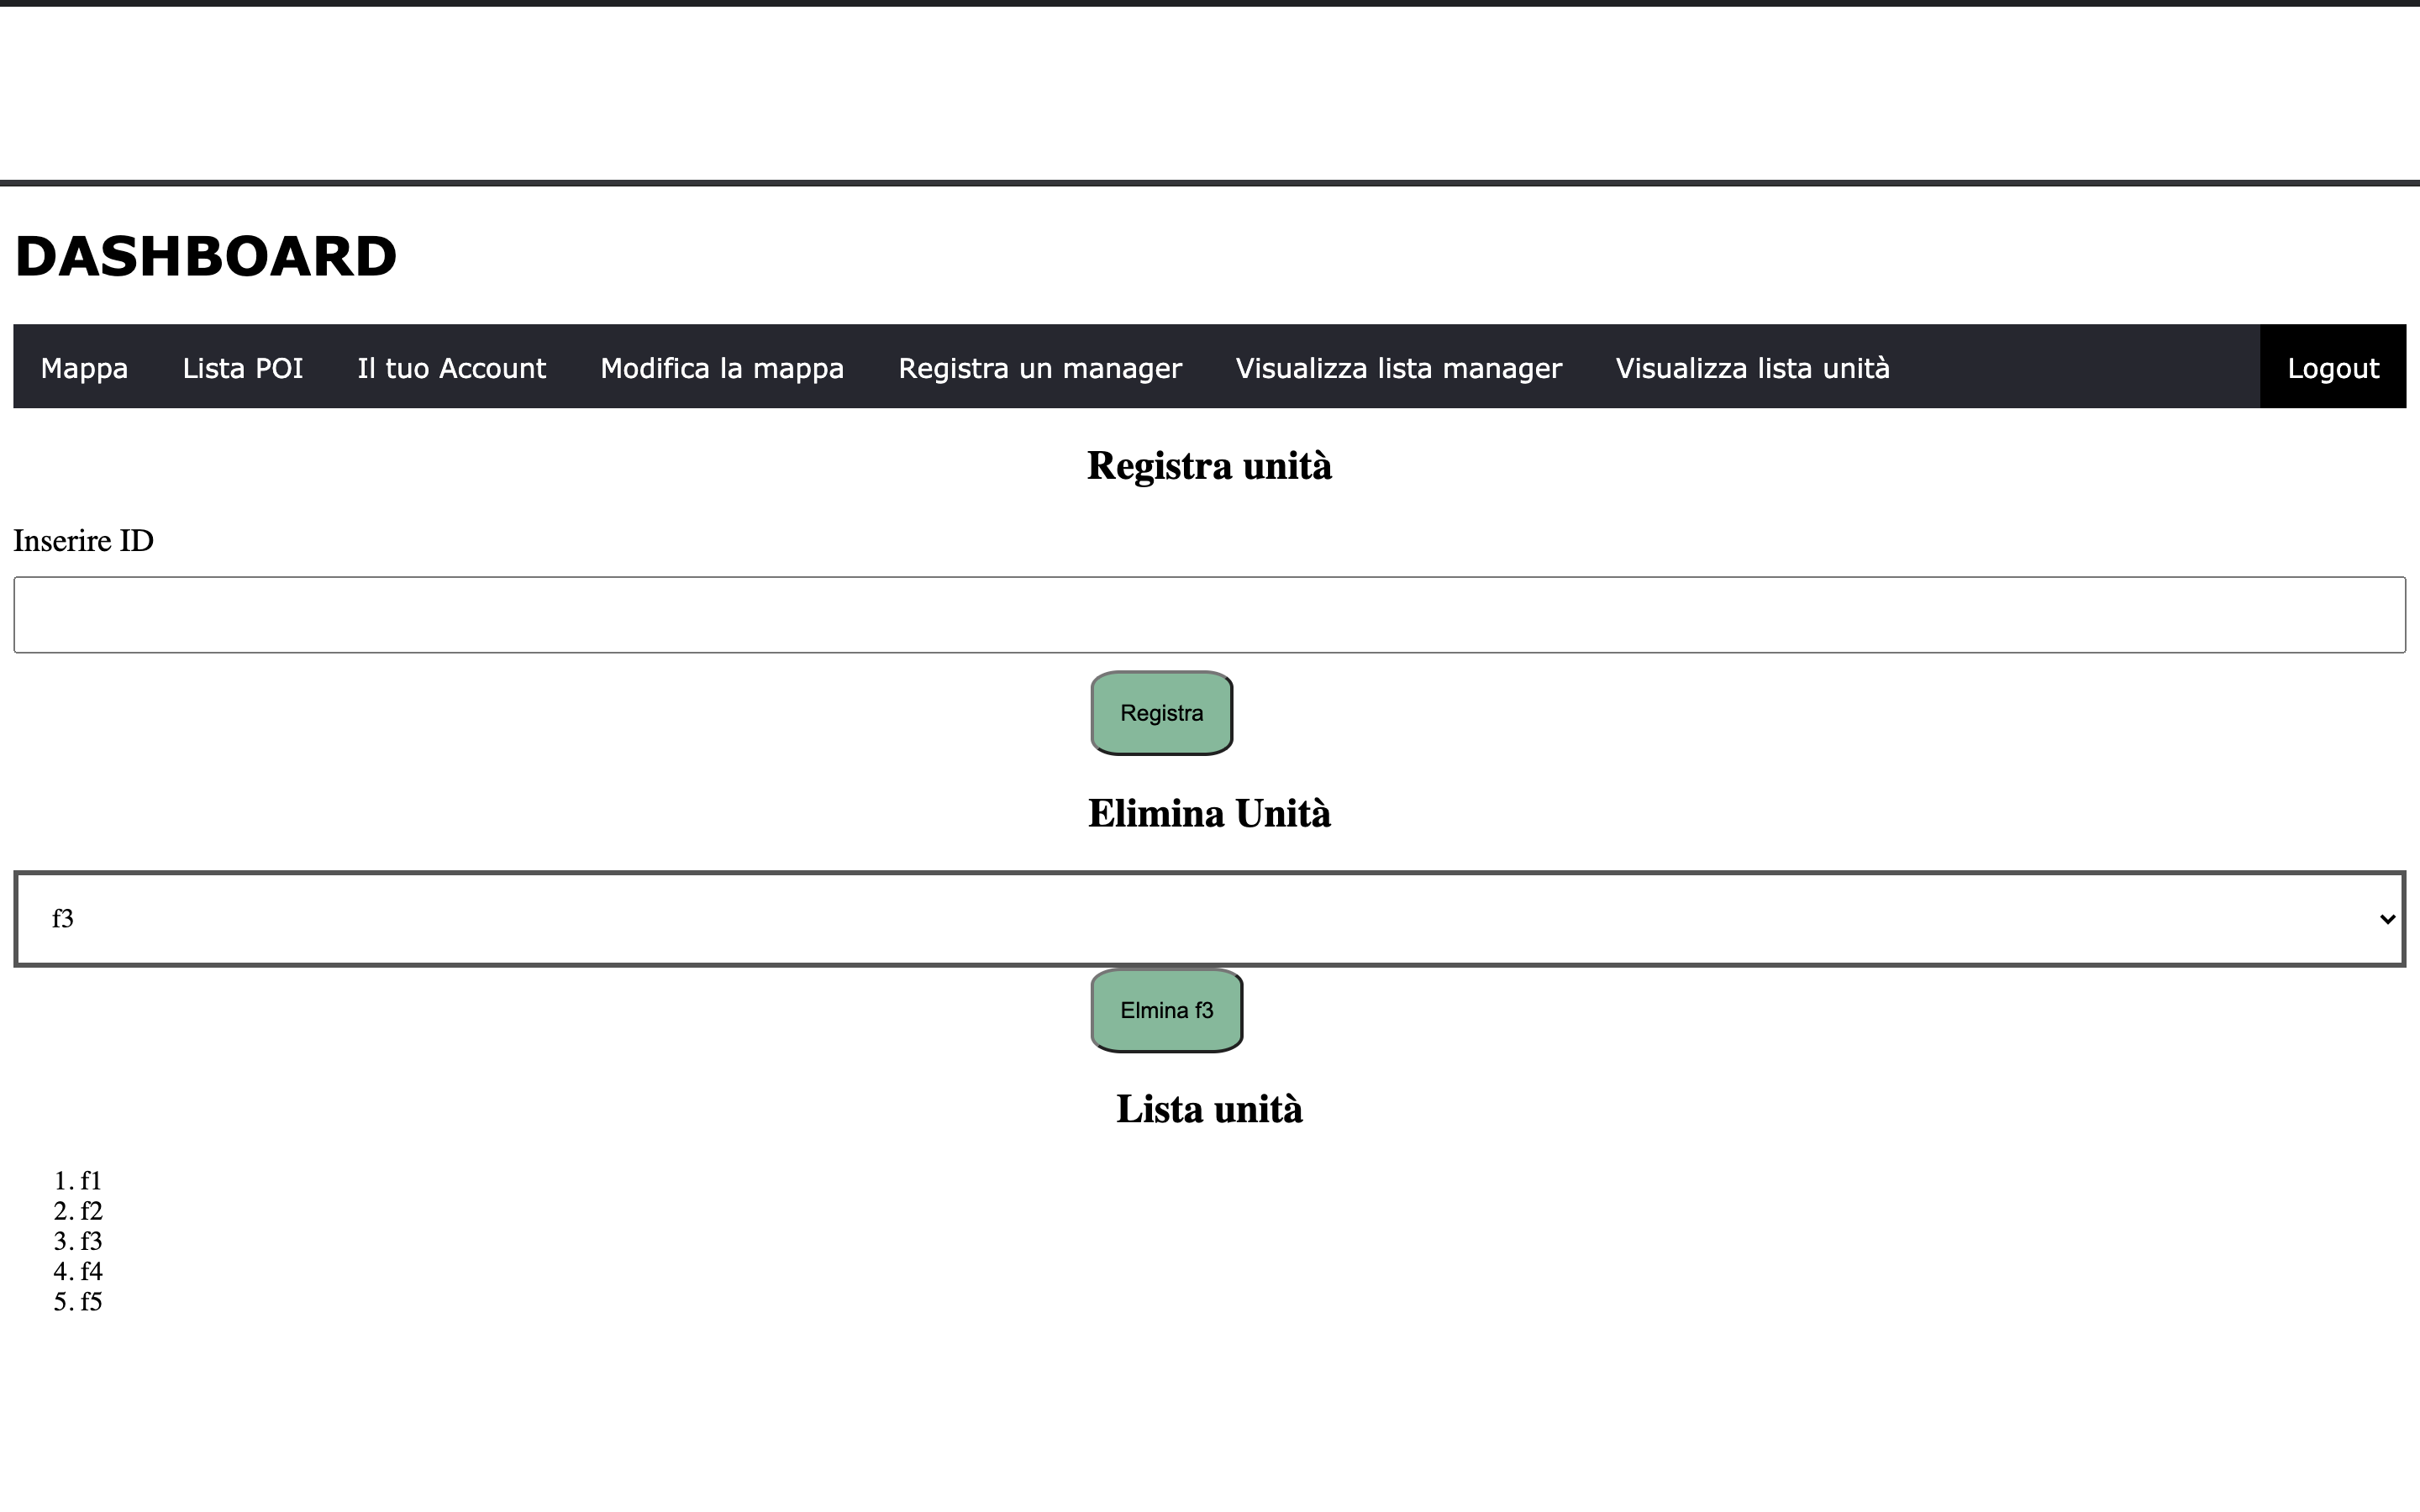
\includegraphics[scale=0.12]{res/images/newunit_admin.png}
    \caption{Schermata guida automatica dell'unità}
\end{figure}